\section*{Problem 3}
Compute the Fourier series for the following signals:

\begin{enumerate}
%%%%%%%%%%%%%%%%%%%% a %%%%%%%%%%%%%%%%%%%%%%
\item $x(t) = 2 + 4 \cos(50t + \pi/2) + 12 \cos(100t-\pi/3)$
\subsection*{Solution}
Lets recall from \cite{kamen2000fundamentals} that:
\begin{equation*}
x(t) = a_0 + \displaystyle\sum_{k=1}^{\infty} A_k \cos(k \omega_0 t + \theta_k) \;
-\infty < t < \infty 
\end{equation*} 

And the equivalent coefficients between the trigonometric series and the 
exponential form are:

\begin{equation}
\begin{aligned}
X_0 &= a_0 \\
|X_n| &= \frac{1}{2} A_k \; , k=1,2,.. \\
\angle X_n &= \theta_k \; , k=1,2,..
\label{eq:c1p31}
\end{aligned}
\end{equation} 

From (\ref{eq:c1p31}) we can immediately calculate the $X_n$ coefficients:
\zcodemat{sources/c1p3a.m}{Plot Magnitude and Angle of $X_n$}

\begin{figure}[H]
\caption{Magnitude and Angle of $X_n$}
\centering
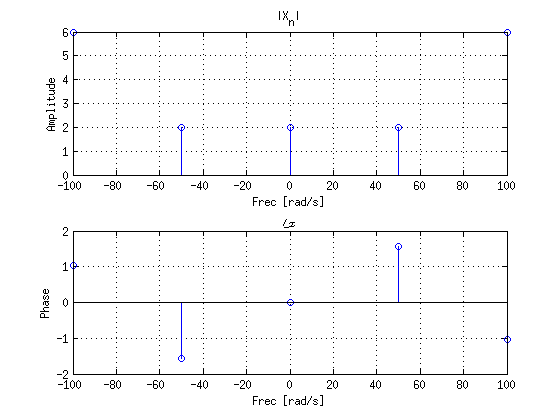
\includegraphics[width=0.8\textwidth]{figs/c1p3a.png}
\label{fig:c1p3a}
\end{figure} 

%%%%%%%%%%%%%%%%%%%% b %%%%%%%%%%%%%%%%%%%%%%
\item $x(t) = 4 \cos(2\pi(1000)t)\cos(2\pi(750000)t)$
\subsection*{Solution}
\begin{equation*}
\begin{aligned}
 x(t) &= 4 \left( \frac{e^{j 2\pi(1000)t} + e^{-j 2\pi(1000)t}}{2} \right)
	  \left( \frac{e^{j 2\pi(750000)t} + e^{-j 2\pi(750000)t}}{2} \right) \\
 &= e^{j 2\pi(751000)t} + e^{j 2\pi(-749000)t} + e^{j 2\pi(749000)t} + e^{j 2\pi(-751000)t}
\end{aligned}
\end{equation*} 

\begin{figure}[H]
\caption{Magnitude and Angle of $X_n$}
\centering
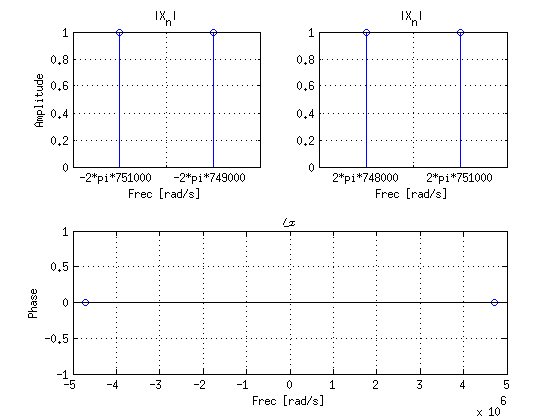
\includegraphics[width=0.8\textwidth]{figs/c1p3b.png}
\label{fig:c1p3b}
\end{figure} 

%%%%%%%%%%%%%%%%%%%% c %%%%%%%%%%%%%%%%%%%%%%
\item The function:
\begin{figure}[H]
\caption*{}
\centering
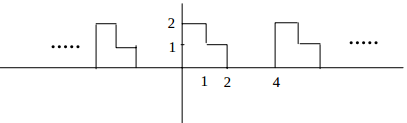
\includegraphics[width=0.7\textwidth]{figs/c1p3e1.png}
\label{fig:c1p3e1}
\end{figure} 

\subsection*{Solution}
The period of the shown signal is $T=4$ and therefore $\omega_0 = \frac{2 \pi}{T} =  \frac{\pi}{2}$.

Taking the derivative of the function we get:
\begin{figure}[H]
\caption{Derivative $\dot{x}$}
\centering
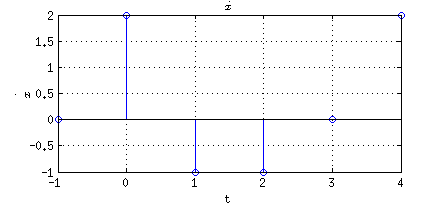
\includegraphics[width=0.8\textwidth]{figs/c1p3c1.png}
\label{fig:c1p3c1}
\end{figure}

In the range $[-1, 3]$ we have:

\begin{equation*}
\dot{x}(t) = 2 \delta(t) - \delta(t-1) - \delta(t-2)
\end{equation*} 

Applying (\ref{eq:c12}) we have:

\begin{equation*}
\begin{aligned}
j n \omega_0 X_n &= \frac{1}{T} \displaystyle\int_{- T/2}^{T/2}
	[2 \delta(t) - \delta(t-1) - \delta(t-2) ]  e^{-j n \omega_0 t} \; dt \\
&=\frac{1}{4} [2 - e^{-j n \frac{\pi}{2}} - e^{n j \pi}]
\end{aligned}
\end{equation*} 

We can use the following properties:
\begin{equation*}
\begin{aligned}
e^{-j n \pi} = (e^{-j \pi})^n = [\cos(\pi) - j \sin(\pi)]^n = (-1)^n \\
e^{-j n \frac{\pi}{2}} = (e^{-j \frac{\pi}{2}})^n 
= [\cos(\frac{\pi}{2}) - j \sin(\frac{\pi}{2})]^n = (-j)^n
\end{aligned}
\end{equation*} 

And reduce the equation to:

\begin{equation*}
X_n =\frac{1}{2 j n \pi} [2 - (-1)^n - (-j)^n]
\end{equation*} 

where 
\begin{equation*}
X_0 = \frac{1}{4} \int_{-1}^{3} x(t) \; dt = \frac{3}{4}
\end{equation*} 

%%%%%%%%%%%%%%%%%%%% d %%%%%%%%%%%%%%%%%%%%%%
\item The function:
\begin{figure}[H]
\caption*{}
\centering
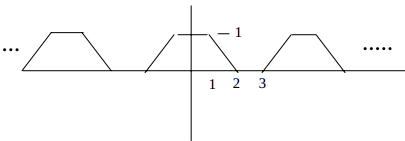
\includegraphics[width=0.7\textwidth]{figs/c1p3e2.png}
\label{fig:c1p3e2}
\end{figure} 

\subsection*{Solution}
The period of the shown signal is $T=5$ and therefore $\omega_0 = \frac{2 \pi}{T} =  \frac{2 \pi}{5}$.

Taking the derivative of the function we get:
\begin{figure}[H]
\caption{First and Second Derivatives $\dot{x}$ $\ddot{x}$}
\centering
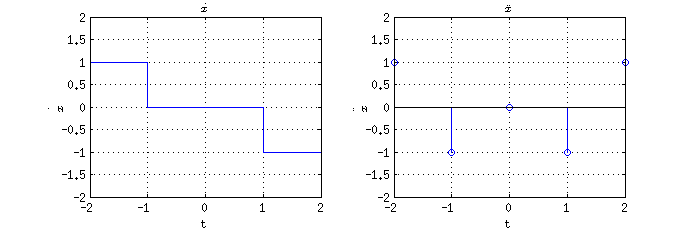
\includegraphics[width=0.8\textwidth]{figs/c1p3d1.png}
\label{fig:c1p3d1}
\end{figure}

In the range $[-2, 2]$ we have:

\begin{equation*}
\ddot{x}(t) = \delta(t+2) - \delta(t+1) - \delta(t-1) + \delta(t-2)
\end{equation*} 

Applying (\ref{eq:c13}) we have:

\begin{equation*}
\begin{aligned}
-n^2 \omega_0^2 X_n &= \frac{1}{T} \displaystyle\int_{- T/2}^{T/2}
	[\delta(t+2) - \delta(t+1) - \delta(t-1) + \delta(t-2)] e^{-j n \omega_0 t} \; dt\\
&=\frac{1}{5} [(e^{2 j n \omega_0} + e^{-2 j n \omega_0}) - 
			  (e^{j n \omega_0} + e^{- j n \omega_0})] \\
X_n &=\frac{2}{5 n^2 \omega_0^2} [\cos(n \omega_0) - \cos(2 n \omega_0)] \\
\end{aligned}
\end{equation*} 

We can calculate the dc component by finding the area of the trapezoid:

\begin{equation*}
\begin{aligned}
X_0 &= \frac{1}{T} \displaystyle\int_{- T/2}^{T/2} x(t) \;dt \\
    &= \frac{1}{5}  \frac{B.b}{2} h = \frac{3}{5}
\end{aligned}
\end{equation*} 

\end{enumerate} 



